\documentclass[../main.tex]{subfiles}
\begin{document}
\setchapterstyle{kao}
\setchapterpreamble[u]{\margintoc}
\chapter[Lie Algebra of a Matrix Lie Group]{Lie Algebra of a Matrix Lie Group\footnotemark[0]}
\labch{Lie-Algebra}
%Continuo LEZIONE 17 05/05
Now we have three powerful tools: the exponential, the logarithm and the polar decomposition of a matrix, or, more generally, an operator. With these tools we want to treat the argument of the \textit{Lie algebra} from a concrete and explicit viewpoint. We already gave the abstract definition of a Lie algebra of a Lie group in the \vrefdef{Lie-algebra}, and we did not insist too much.
\begin{figure}[h!]
    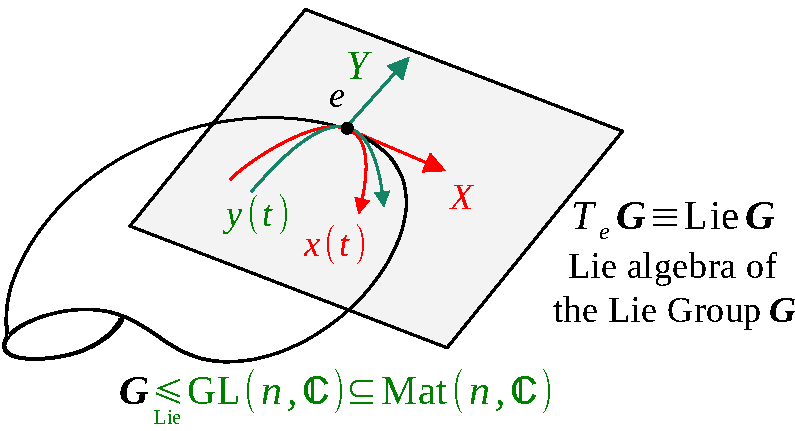
\includegraphics[width=1\textwidth]{images/inf-struct-lie-group2.pdf}
    \caption{Reproposing of \reffig{inf-struct-lie-group}.}
    \labfig{inf-struct-lie-group2}
\end{figure}
In \reffig{inf-struct-lie-group2} it is represented our Lie group $G$, which is a manifold and, as a group, it has a distinguish point, which is the \textit{neutral element} $e$ (which we will call also \textit{identity} having in mind the case of matrices); and, as a manifold, it has a tangent space to the identity $T_eG$. If we now take two tangent vectors to the identity, say $X$ and $Y$, each one of them corresponds, by definition, to a smooth path which is passing through the neutral element at zero. If everything is embedded (\textit{immerso}), as it often happens, we might think that $Y$ and $X$ are, respectively the velocities at time $t=0$ of the paths $y(t)$ and $x(t)$; if the group is not embedded, then, by definition, the two tangent vectors are equivalent classes of paths which include the red and the green ones in the picture. 
\paragraph{Abstract (geometric) viewpoint}:
So, we already have the abstract viewpoint which tells us that since $G$ is a group, we can perform some operations on our path: we can multiply them punt-ways. The idea is that, with the two red and green paths, we can define a new path by taking the inverse, but with also have to rescale time
\[
w(t)={\color{red}x(\sqrt{t})}{\color{Green}y(\sqrt{t})}{\color{red}x(\sqrt{t})^{-1}}{\color{Green}y(\sqrt{t})^{-1}}
\]
This is a path which at zero is at the identity and it is smooth except at zero. We take this path and we take the equivalent class of this path $w$, denoted $\bqty{w}$ and, since it depends on $X=\bqty{x}$ and $Y=\bqty{y}$, we set
\[
{\color{red}\bqty{w}:=\bqty{X,Y} \quad \textrm{Lie brackets}}
\]
There are still many things to prove, for example to prove that this is bilinear and anti-symmetric.\marginnote{But the abstract viewpoint is only half of the cake, because the other half is the concrete viewpoint, which will explain us why we choose exactly the same symbol that we have always been using for the commutator. Indeed, in the concrete case it will be the \textit{commutator}. But what is the concrete case? It is that $G$ is a matrix Lie group (it can be a group of matrices by definition or up to an isomorphism), but a group of matrices is a subgroup of the general linear group for some dimension $n$, which is an open subset of the linear space of all the matrices. So in the concrete case, we have to imagine that \reffig{inf-struct-lie-group2} is embedded in a linear space of dimension $n^2$, therefore the tangent space to the identity is also a linear subspace of this large linear space of dimension $n^2$, in which the point are matrices.}
\paragraph{Concrete viewpoint}: As $G\leq \textrm{GL}(n,\mathbb{C})$ for some $n\in\mathbb{N}$, everything is embedded in the \underline{\underline{\textbf{linear space}}} $\textrm{Mat}(n,\mathbb{C})\cong \mathbb{R}^{2n^2}$. Here we can compute derivatives as the limit of the incremental ratio (we are allowed to take differences and ratios since everything is embedded).
\[
X=\lim_{\varepsilon\to 0}\overset{\mathclap{\tikz \node {$\downarrow$} node [above=1.25ex] {\footnotesize $\ $ ok};}}{\frac{1}{\varepsilon}}(x(\varepsilon)\overset{\mathclap{\tikz \node {$\downarrow$} node [above=1.25ex] {\footnotesize $\ $ ok};}}{-}\mathbb{1})=\dv{t}x(t)\big|_{t=0}\qquad \textrm{in Mat}(n,\mathbb{C})
\]
We do not need anymore to define $X$ as the equivalence class of all the paths which are passing through the neutral element at time zero and are tangent to each other.

As pedagogical choice, instead of going from the abstract to the concrete, we will now do the opposite. We define a matrix Lie algebra (following more or less Chapter 3 of \sidecite{Hall2015_Ch3}) and then we will have some results and we will discover that the matrix Lie algebra is the Lie algebra (in the geometric abstract sense) of the (matrix) Lie group
\[
\text{\parbox{4 cm}{\centering (matrix)\\[1pt] Lie algebra \\[1pt]  {\color{Green} (concrete)}\\[1pt] $X$}}\text{\parbox{1cm}{$\overset{\cong}{\leftrightsquigarrow}$\\[14pt] $\leftrightsquigarrow$}}\text{\parbox{4 cm}{\centering Lie algebra\\[1.5pt] of the Lie group \\[1.5pt]  {\color{Green} (abstract)}\\[1pt] $\bqty{e^{tX}}\in T_{\mathbb{1}}$}}
\]
\section{Definition and basics}
\underline{Hp:} Let $G$ be a \textbf{matrix} Lie group, i.e. $G\underset{\textrm{Lie}}{\leq}\textrm{GL}(n,\mathbb{C})$\marginnote{We put the word \textit{matrix} in brackets because at some point we will understand that it is THE Lie algebra

The symbol $\mathfrak{g}$ is made with the command $\backslash$mathfrak\{g\}
}
\begin{definition}[(Matrix) Lie algebra]\index{Lie algebra}The \textbf{(matrix)} Lie algebra of $G$, denoted as $\textrm{Lie}\;G$ or $\mathfrak{g}$, is
\[
\mathfrak{g}=\big\{X\in\textrm{Mat}(n,\mathbb{C}):\ e^{tX}\in G \ \underbrace{\underline{\underline{\forall\;t\in\mathbb{R}}}}_{\textrm{For every $t\in\mathbb{R}$!}}\big\}
\]
\end{definition}
If $G$ is the general linear group, then $e^{tX}$ is in the general linear group (is invertible) for every $t$ and then the matrix Lie algebra will be all the matrices. This corresponds to the fact that the general linear group is \textbf{flat}. So we take an open subset of a flat space, the tangent space to this open flat subset is the full linear space. But now imagine that $G$ is not the general linear group, but it is the special linear group; then we are asking that $e^{tX}$ is in the special linear group, i.e. it has the determinant equal to one for every time. From this it will follow (see after) the condition that the trace of $X$ should be zero. Now suppose that $G$ is even smaller: it is the unitary group; then we have a constraint: at every time we want $e^{tX}$ to be unitary, but this will be a constraint on $X$ and we will discover that $X$ should be anti-self-adjoint in the notation of mathematicians, or self-adjoint in the physicists' one.
\begin{proposition}
Let $G$ be a matrix Lie group, and take $X$ in the corresponding matrix Lie algebra $X\in\mathfrak{g}$. Then ${\color{red}e^X\in G_\circ}$, where $G_\circ$ is \textbf{identity component of $G$}.
\end{proposition}
So if we take a vector in the Lie algebra and we take the exponential of it, we will always stay in the connected components at the identity; we will never reach the other connected components.
\begin{proof}
Take the map $\bqty{0,\;1}\ni t \mapsto e^{tX}\overset{\mathclap{\tikz \node {$\downarrow$} node [above=1.25ex] {\footnotesize $X$ is in the Lie algebra};}}{\in}G$. Let us give a name to it:
\begin{marginfigure}
	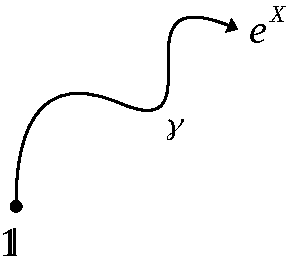
\includegraphics[width=1\linewidth]{images/matrix-lie-algebra.pdf}
	\caption[Arcwise connected path]{}
	\labfig{dim-prop-matrix-lie-group}
\end{marginfigure}
\[
\gamma(t)=e^{tX}\xrightarrow[]{}\begin{cases}
    \gamma(0)&=\mathbb{1}\\
    \gamma(1)&=e^{X}
\end{cases}
\]
The path is continuous (even smooth), so we found a path $\gamma$ in \reffig{dim-prop-matrix-lie-group} from the identity to $e^{X}$, so it means that $e^{X}$ is arc-wise connected to the identity. And then it should be in the same connected component.
\end{proof}
The moral is that we cannot pretend to reach every element of the group by exponentiating elements of the Lie algebra, we will only reach elements inside the identity component of the group, all the others are lost somewhere else.\marginnote{It is not even obvious that we can reach all of them.}
\begin{proposition}
Let $G$ be a matrix Lie group, $\mathfrak{g}=\textrm{Lie}\;G$. For every $X,Y\in\mathfrak{g}$, the following properties hold true:
\renewcommand{\labelenumi}{\arabic{enumi})}
\begin{enumerate}
    \item $A\cdot X\cdot A^{-1}\in\mathfrak{g}\quad\forall\;A\in G$\marginnote{Notice that this is multiplication of matrices, in abstract it will make no sense to multiply an element of the group with the tangent vector at the identity. But if everything is a matrix, it is ok}
    \item $sX\in\mathfrak{g}\quad \forall\;s\in\mathbb{R}$ \textbf{(real!)}
    \item $X+Y\in\mathfrak{g}$
    \item $XY-YX\in \mathfrak{g}$
\end{enumerate}
2) + 3) tells us that $\mathfrak{g}$ is a linear space. 4) tells us that the Lie algebra is left invariant by taking the commutators of the elemetns.
\end{proposition}
\begin{proof}
\renewcommand{\labelenumi}{\arabic{enumi})}
\begin{enumerate}
    \item Is $e^{tAXA^{-1}}\in G\quad \forall\;t\in\mathbb{R}$? Let us compute it.\marginnote{$e^{tX}$ is in the group by definition of matrix Lie algebra, while $A$ and $A^{-1}$ are both in $G$ by our choice}
    \[
    e^{tAXA^{-1}}=e^{A(tX)A^{-1}}=\overset{\mathclap{\tikz \node {$\downarrow$} node [above=1.25ex] {\footnotesize in $G$};}}{A}\underbrace{e^{tX}}_{\in G\;\forall t\in\mathbb{R}}\overset{\mathclap{\tikz \node {$\downarrow$} node [above=1.25ex] {\footnotesize in $G$};}}{A^{-1}}
    \]
    The product of elements in the group, is in the group, therefore:
    \[
    e^{tAXA^{-1}}\in G\quad \forall\;t\in\mathbb{R}
    \]
    \item $e^{t(sX)}=e^{(ts)X}\in G\quad \forall\;t\in\mathbb{R}$
    \item This is the most interesting one. We have to prove that $e^{t(X+Y)}\in G\;\;\forall\;t\in\mathbb{R}$. This is not completely obvious, because the operation in the group is the multiplication of matrices and we know that the exponential of the sum is \textbf{not} the product of the exponentials. We have to find a way to convert\marginnote{We know that it is true if $X$ and $Y$ commute, but this is not the case here}
    \[
    \text{\parbox{4 cm}{\centering exponential\\[1pt] of sums}}\xrightarrow[\textrm{{\color{red}Lie product formula}}]{}\text{\parbox{4 cm}{\centering product of\\[1.5pt] exponentials }}
    \]
    and this is true when the evolution time of the Lie product formula is small. The Lie product formula has been invented exactly for that
    \[
    \underbrace{e^{t(X+Y)}}_{\parbox{1.6cm}{\footnotesize is invertible\\[1pt]is in $\textrm{GL}(n,\mathbb{C})$}}=\lim_{m\to+\infty}\underbrace{\Big(\underbrace{e^{\frac{t}{m}X}}_{\textrm{in }G}\underbrace{e^{\frac{t}{m}Y}}_{\textrm{in }G}\Big)^m}_{\textrm{in }G}
    \]
    When taking the limit, we use the fact that a matrix Lie group is \textbf{closed in} $\textrm{GL}(n,\mathbb{C})$: the limit either is in $G$, or is not invertible. Hence, the limit \textbf{exists in} $G$, for every $t\in\mathbb{R}$.
    \item Would it be true that $XY-YX\in\mathfrak{g}$?
    
    Take $Y$ and conjugate it with $e^{tX}$:\marginnote{In differential calculus for matrix valued functions (even operators), we still have the Leibniz rule (it is one of the recommended exercise)}
    \[
    \dv{t}e^{tX}Ye^{-tX}\big|_{t=0}\overset{\mathclap{\tikz \node {$\downarrow$} node [above=1.25ex] {\footnotesize Leibniz rule};}}{=}\left[e^{tX}XYe^{-tX}+e^{tX}Y(-X)e^{-tX}\right]_{t=0}=XY-YX
    \]
    {\fontencoding{U}\fontfamily{futs}\selectfont\char 66\relax} We learned that the commutator $\comm{X}{Y}$ is the \textbf{infinitesimal form} of the action by conjugation with $e^{tX}$\marginnote{In a sense this is the reason why commutator appears in quantum mechanics}
    \[
    \dv{t}e^{tX}Ye^{-tX}\big|_{t=0}=XY-YX
    \]
    We prefer to write
    \[
    XY-YX=\lim_{\varepsilon\to 0}\underbrace{\frac{1}{\varepsilon}\Big(\underbrace{e^{\varepsilon X}Ye^{-\varepsilon X}}_{\in\;\mathfrak{g}\textrm{ by (1)}}-\underbrace{Y}_{\in\;\mathfrak{g}}\Big)}_{\in\mathfrak{g} \textrm{ by (2) and (3)}}
    \]
    Now we are done, because : $Y$ lives in the Lie algebra from the beginning; $e^{\varepsilon X}Ye^{-\varepsilon X}$ is in the Lie algebra by point (1); the Lie algebra is a linear space by point 2) and 3) and, since the Lie algebra is a finite dimensional linear space $\dim\mathfrak{g}<+\infty$, hence $\mathfrak{g}$ it is \textbf{closed} and therefore the limit is still in the Lie algebra $\mathfrak{g}$.
\end{enumerate}
\end{proof}
%1:29:13
%INIZIO LEZIONE 06/05
\section{Lie algebra of classical Lie groups}
\labsec{importancei}
\subsection{Warning: The importance of being $i$}\marginnote{This could be a subtle reference to \href{https://www.youtube.com/watch?v=jySfU10IQu4}{Oasis} or to \href{https://en.wikipedia.org/wiki/The_Importance_of_Being_Earnest}{Oscar Wilde}. Thanks to Silvio for pointing this out. The literature on the subject is schizophrenic}
{\fontencoding{U}\fontfamily{futs}\selectfont\char 66\relax} Mathematicians and physicists never found an agreement on what is relevant:
\[
\begin{cases}
\text{Mathematicians:} \quad &U=e^X\Rightarrow X^*=-X \\
\text{Physicists:} \quad &U=e^{\color{red}iG}\Rightarrow{\color{red}G^*=G}
\end{cases}
\]
The two are equivalent if we take $X=iG$. The advantages of the physics notation are that it is coherent with \href{https://en.wikipedia.org/wiki/Erwin_Schr\%C3\%B6dinger}{Schr\"odinger}'s dynamics $U(t)=e^{iH}$ and with the fact that, since $G$ is self adjoint, we get that $G$ is an observable itself.

Since this course is labelled MAT/07 and since we will follow books written by mathematicians, we will follow the math notation.
\begin{marginfigure}[-25mm]
	\includegraphics[width=1\linewidth]{images/Erwin_Schrödinger_(1933).jpg}
	\caption[Photo of Schrödinger]{From \href{https://commons.wikimedia.org/wiki/File:Erwin_Schr\%C3\%B6dinger_(1933).jpg}{Wikimedia}: Erwin Rudolf Josef Alexander Schrödinger (12 August 1887 – 4 January 1961), was a Nobel Prize-winning Austrian-Irish physicist who developed a number of fundamental results in quantum theory: the Schrödinger equation provides a way to calculate the wave function of a system and how it changes dynamically in time. He died in Vienna of tuberculosis at the age of 73.}
	\labfig{Schrodinger}
\end{marginfigure}
\subsection{General and Special linear group}
\begin{proposition}\labprop{GLSL}
For the general and the special linear group we have:
\renewcommand{\labelenumi}{\Roman{enumi})}
\begin{enumerate}
    \item Lie GL$(n,\mathbb{C})=\text{Mat}(n,\mathbb{C})\equiv\mathfrak{gl}(n,\mathbb{C})$
    \item Lie GL$(n,\mathbb{R})=\text{Mat}(n,\mathbb{R})\equiv\mathfrak{gl}(n,\mathbb{R})$
    \item Lie SL$(n,\mathbb{C})=\{X\in\text{Mat}(n,\mathbb{C}):{\color{red}\tr(X)=0}\}\equiv\mathfrak{sl}(n,\mathbb{C})$
    \item Lie SL$(n,\mathbb{R})=\{X\in\text{Mat}(n,\mathbb{R}):{\color{red}\tr(X)=0}\}\equiv\mathfrak{sl}(n,\mathbb{R})$
\end{enumerate}
\end{proposition}
\begin{proof}
The fact that the Lie algebra of the general linear group is the whole linear space of matrices, corresponds to the geometric idea that the general linear group is flat.
\renewcommand{\labelenumi}{\Roman{enumi})}
\begin{enumerate}
    \item $\forall\, X\in\text{Mat}(n,\mathbb{C})$ we already proved that $e^{tX}$ is invertible hence it is in GL$(n,\mathbb{C})$. More specifically, we even know that \[\left(e^{tX}\right)^{-1}=e^{-tX}\]
    \item $\forall\, X\in\text{Mat}(n,\mathbb{R})$ we have that $e^{tX}$ is invertible and \underline{\textbf{real}} so it is in GL$(n,\mathbb{R})\;\forall t\in\mathbb{R}$. Vice versa, suppose that $e^{tX}\in\textrm{GL}(n,\mathbb{R}) \ \forall\; t\in\mathbb{R}$. We observe that:
    \[
    X=\dv{t}e^{tX}\Bigr|_{\substack{t=0}} \ \text{is in Mat}(n,{\color{red}\mathbb{R}})
    \]
    \item $\forall X\in\mathfrak{sl}$ (in particular $(n,\mathbb{C})$), {\color{red}$\tr(X)=0$}. Then, 
    \[
    \det\left(e^{tX}\right)\underset{\mathclap{\tikz \node {$\uparrow$} node [below=1ex] {\footnotesize  magic formula of \vrefthm{MagicFormula}};}}{=}e^{t\tr(X)}=e^0=1
    \]
    Vice versa, suppose to have $\det\left(e^{tX}\right)=1\ \forall\; t\in\mathbb{R}$:
    \[
    1=\det\left(e^{tX}\right)\underset{\mathclap{\tikz \node {$\uparrow$} node [below=1ex] {\footnotesize  magic formula};}}=e^{t\tr(X)}\;\xrightarrow[\text{differentiation}]{}\;0=\dv{t}e^{t\tr(X)}\Bigr|_{\substack{t=0}}=\tr(x)
    \]
    \[
    \Rightarrow\quad \tr(X)=0
    \]
    \item Combination of arguments from II) and III).
\end{enumerate}
\end{proof}
\subsection{Unitary and Special unitary group}
\begin{proposition}\labprop{USUOSO}
For the unitary and the special unitary group we have:
\renewcommand{\labelenumi}{\Roman{enumi})}
\begin{enumerate}
\item Lie U$(n)=\{X\in\text{Mat}(n,\mathbb{C}):{\color{red}X^*=-X}\}\equiv\mathfrak{u}(n)$
\item Lie SU$(n)=\{X\in\text{Mat}(n,\mathbb{C}):X^*=-X, \tr(X)=0\}\equiv\mathfrak{su}(n)$
\item Lie O$(n)=\{X\in\text{Mat}(n,\mathbb{R}):{\color{red}\underbrace{X^T=-X}_{\textrm{Anti-symmetric matrix}}}\}\equiv\mathfrak{o}(n)$\marginnote{Anti-symmetric matrices $ \Rightarrow\tr(X)=0$}
\item Lie $\textrm{SO}(n)=\textrm{Lie}\, \textrm{O}(n)$
\end{enumerate}
\end{proposition}
Why in the last line there is no additional condition?
\begin{marginfigure}
    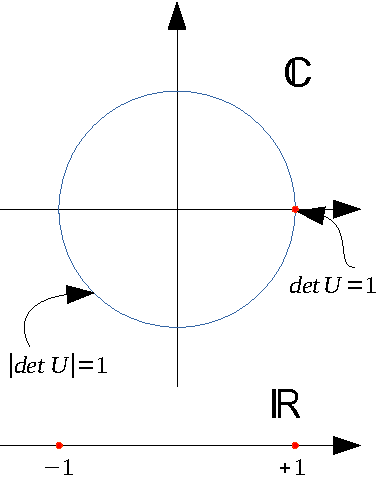
\includegraphics[width=1\linewidth]{images/u(n)su(n)o(n)so(n).pdf}
	\caption{The circle is from $\mathfrak{u}(n)$ to $\mathfrak{su}(n)$, the line is from $\mathfrak{o}(n)$ to $\mathfrak{so}(n)$.} %RIVEDERE ALCUNE COSE IMMAGINE
	\labfig{usuoso}
\end{marginfigure}
\underline{\textbf{Remark:}} In U$(n)$ we have that $|\det U|=1$, while in $\textrm{SU}(n)$ we have $\det U=1$. $\textrm{SU}(n)$ is a codimension-1 subgroup of U$(n)$, correspondingly, dim SU$(n)=\dim \textrm{U}(n)-1$. On the other hand, we have that $\det R\in\{-1,+1\}$ for every $R$ in O$(n)$. Instead, for $R\in\textrm{SO}(n)$ we have that $\det R=+1$: we exclude a point which has dimension zero, so we do not need an additional constraint for $\textrm{SO}(n)$.

Moreover, we already know that the special orthogonal group (at least, we have seen it in dimension three) is the identity component of the orthogonal group; and from the geometric picture it is clear that the Lie algebra depends only on what happens near the identity: because the Lie algebra is the tangent space to the identity and the Lie algebra structures come from multiplication of paths, which at time zero are at the identity. Hence, what happens in the other connected components is completely irrelevant to the Lie algebra. Take the orthogonal group in three dimensions: $\textrm{O}(3)$, it has two connected components, one is around the identity and the other is around minus the identity. The Lie algebra does not know anything about what happens around minus the identity, because the Lie algebra is completely characterized by the local structure in a small neighbourhood around the identity, what happens far away is not interesting to the definition of the Lie algebra. Again, this is a second argument to see that is not surprising to see that $\textrm{O}(3)$ has the same Lie algebra of $\textrm{SO}(3)$.

There is a third argument: if we are in the Lie algebra of $\textrm{O}(n)$, we are dealing with antisymmetric matrices, and antisymmetric matrices have zero diagonal, so it is obvious that the trace is zero.
\begin{proof}
\renewcommand{\labelenumi}{\Roman{enumi})}
\begin{enumerate}
\item $\forall X\in\mathfrak{u}(n)$, we have that $e^{tX}$ is unitary $\forall\;t\in\mathbb{R}$: indeed we see that
\[
e^{tX}\left(e^{tX}\right)^*\underset{\mathclap{\tikz \node {$\uparrow$} node [below=1ex] {\footnotesize 2) of \refprop{exp-prop} };}}=e^{tX}e^{t{\color{red}X^*}}=e^{tX}e^{\color{red}-tX}=\mathbb{1}
\]
Vice versa, suppose $e^{tX}\in \textrm{U}(n)\ \forall\;t\in\mathbb{R}$:\marginnote{The proof of the Leibniz rule was a recommended exercise}
\WithArrowsOptions{displaystyle}
\[
\begin{WithArrows}
\mathbb{1}&=e^{tX}\left(e^{tX}\right)^*\quad \forall t\in\mathbb{R}\Arrow{\text{by Leibniz rule}}\\
0&=\left(Xe^{tX}e^{tX^*}+e^{tX}e^{tX^*}X^*\right)\Bigr|_{\substack{t=0}}\\
\Rightarrow\quad {\color{red}X+X^*}&={\color{red}0} \quad \textrm{for }t=0
\end{WithArrows}
\]
\item As in \refprop{GLSL} for $\mathfrak{sl}(n,\mathbb{C})$\\
\item If $X\in\mathfrak{o}(n)$, is $e^{tX}\in\textrm{O}(n)\ \forall\; t\in\mathbb{R}$? We have to check that $e^{tX}\left(e^{tX}\right)^T=\mathbb{1}$ (in finite dimension we have to check just one of the equalities, in infinite dimension both).\marginnote{The tools are more or less the same: Leibniz rule, properties of the exponential}

\underline{\textbf{Claim: }} $(e^{tX})^{\color{red}T}=e^{tX^{{\color{red}T}}}$ for \textbf{real} matrices $X$:
\[
\left(e^{tX}\right)^T\underset{X\textrm{ real}}{=}(e^{tX})^*\overset{\mathclap{\tikz \node {$\downarrow$} node [above=1.25ex] {\footnotesize 2) of \refprop{exp-prop}};}}{=}e^{tX^*}\underset{X\textrm{ real}}{=}e^{tX^T}
\]
Now we are ready to conclude that for an anti-symmetric (and so also self-adjoint) matrix:
\[
e^{tX}(e^{tX})^T=e^{tX}e^{t{{\color{red}X^T}}}\underset{\mathclap{\tikz \node {$\uparrow$} node [below=1ex] {\footnotesize $XX^T=-X^2=X^TX$ };}}=e^{t(X+X^T)}=e^0=\mathbb{1}
\]
Vice versa, suppose to have $e^{tX}\in\textrm{O}(n)\ \forall\; t\in\mathbb{R}:$
\[
\mathbb{1}=e^{tX}(e^{tX})^T=\dots=e^{t(X+X^T)} \quad \forall t\in\mathbb{R}
\]
Since it is true for every $t$, we differentiate for $t=0$:
\[
0=\dv{t}e^{t(X+X^T)}\Bigr|_{\substack{t=0}}=X+X^T\quad \Rightarrow\ X^T=-X
\]
\item By the magic formula, the constraint $\det e^X=1$ corresponds, in both directions, to $\tr(X)=0$. But as $X$ is \textbf{anti-symmetric} $\left(X^T=-X\right)$, its trace is automatically zero: Lie SO$(n)=\mathfrak{o}(n)\equiv\mathfrak{so}(n)$
\end{enumerate}
\end{proof}
\subsection{Orthogonal and Special orthogonal group}
We recall that O$(p,q)$ is the set of $\Lambda\in\textrm{End}(\mathbb{R}^{p+q})$ such that \begin{equation}\labeq{iso}
(\textrm{ISO}) \qquad (\Lambda v|\Lambda w)_g=(v|w)_g \qquad \forall\; v,w\in\mathbb{R}^{p+q}
\end{equation}
with $(v|w)_g=\sum_{i,j}g_{ij}v^iw^j$ and $g_{ij}$ defined as in \refsec{GOG}, with $p$ positive eigenvalues and $q$ negative ones. In particular, O(1,3) is the \textbf{Lorentz group}.\marginnote{
\[
G=\mqty(\dmat{-1,\ddots,-1,+1,\ddots,+1})
\]
}
\begin{proposition}\labprop{GOG} For the general and special orthogonal group we have:
\renewcommand{\labelenumi}{\arabic{enumi})}
\begin{enumerate}
\item Lie O$(p,q)=\left\{X\in\text{Mat}(p+q,\mathbb{R}):{\color{red}GX^TG=-X}\right\}\equiv\mathfrak{o}(p,q)$
\item Lie SO$(p,q)=\textrm{Lie O}(p,q)$
\end{enumerate}
\end{proposition}
\begin{proof}
We translate the (ISO) condition stated in \refeq{iso} into a matrix identity:
\[
(\Lambda v|\Lambda w)_g=\sum_{i,j}g_{ij}\Lambda^i_{\;l}v^l\Lambda^j_{\;m}w^m\overset{\textrm{(ISO)}}{=}(v|w)_g=\sum_{l,m}g_{lm}v^lw^m \quad \forall\; v,w\in\mathbb{R}^{p+q}
\]
By the arbitrariness of $v$ and $w$ we get:
\[
\sum_{i,j}g_{ij}\Lambda^i_{\;\;l}\Lambda^j_{\;\;m}=g_{lm} \quad \forall\; l,m
\]
On the left hand side it is clearly a matrix multiplication, but we have to check that the indices are in the correct order\marginnote{We have to add the $\Lambda^T$ because the index $i$ is in the wrong side. Indeed, it is important not also if the index is upstairs or downstairs, but also if it is on the left or right (there is a space!)}
\begin{equation}\labeq{cond-group}
(\Lambda^T)^i_{\;\;l}g_{ij}\Lambda^j_{\;\;m}=g_{lm}\quad \Rightarrow{\color{red}\boxed{\Lambda^TG\Lambda=G} \quad \star}
\end{equation}
This is the condition for a matrix $\Lambda$ to be in the Lorentz group (in general in the generalized orthogonal group). Suppose now that $\Lambda(t)=e^{tX}$ satisfies $(\ref{eq:cond-group})$ $\forall t\in\mathbb{R}$, i.e. $(e^{tX})^TGe^{tX}=G$ $\forall t\in\mathbb{R}$. By Leibniz rule (at $t=0$), we obtain:
\begin{equation}\labeq{GOG-1}
\left(e^{tX^T}X^TGe^{tX}+e^{tX^T}GXe^{tX}\right)\Bigr|_{\substack{t=0}}=0=X^TG+GX \quad (\#\#)
\end{equation}
Now we exploit the fact that is special {\color{red}$G^2=\mathbb{1}, G^{-1}=G$}. Multiplying times $G$ on the left in \refeq{GOG-1} we get:
\begin{equation}\labeq{GOG2}
GX^TG+G^2X=0\quad \Rightarrow \ {\color{red}GX^TG=-X \quad (\#)}
\end{equation}
Vice versa, suppose that $X\in\mathfrak{o}(p,q)$, i.e. it satisfies (\ref{eq:GOG2}). Equivalently, $X^T=-GXG=-GXG^{-1}$. Check that the condition for the group (\ref{eq:cond-group}) for $\Lambda(t)=e^{tX}$:
\[
\left(e^{tX}\right)^TGe^{tX}=e^{t({\color{red}-GXG^{-1}})}Ge^{tX}=G{\color{Green}e^{-tX}}{\color{blue}G^{-1}}{\color{blue}G}{\color{Green}e^{tX}}=G
\]
\end{proof}
\subsection{Symplectic group}
We recall that $\textrm{Sym}(n,\mathbb{R})$ consists of those $A\in\textrm{End}(\mathbb{R}^{2n})$ such that:
\[
\omega(Av,Aw)=\omega(v,w)
\]
And $\omega$ can be written as
\[
\omega(v,w)=\sum_{i,j}\Omega_{ij}v^iw^j \quad \text{ with }\ \Omega=
\left(
\begin{array}{c:c}
    0 & +\mathbb{1} \\
    \hdashline
    -\mathbb{1} & 0
\end{array}
\right)
\]
\begin{proposition}
Lie $\text{S}_\text{p}(n,\mathbb{R})=\{X\in\text{Mat}(2n,\mathbb{R}):\Omega X^T\Omega=X\}$
\end{proposition}
\begin{proof}
The proof is left as an exercise for the reader and it is similar to \refprop{GOG} but with {\color{red}$\Omega^2=-\mathbb{1}$} and {\color{red}$\Omega^T=-\Omega$}.
\end{proof}
\section{Induced Lie algebra homomorphisms}\marginnote{Want to explain that an homomorphism of Lie groups, induces an homomorphism of Lie algebras}
\begin{definition}[Homomorphism of Lie algebras]\index{Homomorphism of Lie algebras}
Suppose $\mathfrak{g}$ and $\mathfrak{h}$ are Lie algebras. An \textbf{homomorphism of Lie algebras} is a map $\psi:\mathfrak{g}\xrightarrow[]{}\mathfrak{h}$ such that:
\renewcommand{\labelenumi}{\Roman{enumi})}
\begin{enumerate}
\item $\psi$ is linear ($\mathbb{R}$-linear);
\item it preserves the Lie brackets, i.e. $\psi([X,Y]_\mathfrak{g})=\comm{\psi(X)}{\psi(Y)}_\mathfrak{h}$
\end{enumerate}
\end{definition}
This is in general, now we want to apply it to our setting:
\[
\phi={\color{red}\textrm{d}}\Phi\big|_e:T_eG\xrightarrow[\textrm{linear}]{}T_eH
\]
\begin{figure}[H]
    \centering
    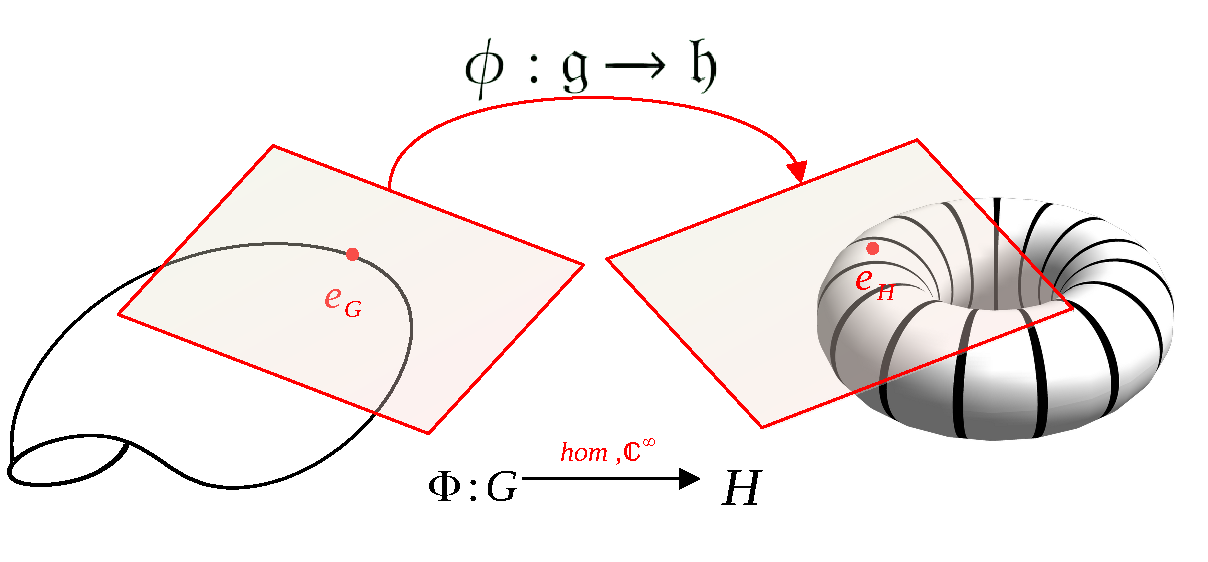
\includegraphics{images/map_homo.pdf}
    \caption{Homomorphism of groups. Manca una descrizione in alto(?).}
    \labfig{map_homo}
\end{figure}
In other words, if we have an homomorphism of Lie groups, its tangent map (or differential as we call it in vectorial Analysis) is a linear map between the tangent space at $G$ and the tangent space at $H$; this is already known. But do we let preserve the Lie brackets or not? Yes, we do! In fact, an homomorphism of Lie groups induces automatically an homomorphism of Lie algebras, essentially in the way which is explained in the \reffig{map_homo} and that we are going to rephrase in another language.
\begin{theorem}[Induced homomorphisms]\index{Induced homomorphisms}
\labthm{ind-homo}
Let $G$ and $H$ be (matrix) Lie groups with $\textrm{Lie}\;G=\mathfrak{g}$ and $\textrm{Lie}\;H=\mathfrak{h}$. Let 
\[
\Phi:G\xrightarrow[]{{\color{red}\text{hom},C^{\infty}}}H
\]Then, there exists a \textbf{unique $\mathbb{R}$-linear map}:
\[
\phi:\mathfrak{g}\xrightarrow[]{}\mathfrak{h}
\]
which satisfies {\color{red}$\Phi( e^X)=e^{\phi(x)}\quad$ (D)}.\\ Moreover:\marginnote{"(D)" is just to mark the property and to be able to refer to it later on, it stands for \textit{\textbf{D}efining property}}
\renewcommand{\labelenumi}{\arabic{enumi})}
\begin{enumerate}
\item $\phi([X,Y])=[\phi(X),\phi(Y)] \qquad\qquad \forall X,Y\in\mathfrak{g}$
\item $\phi(AXA^{-1})=\Phi(A)\phi(X)\Phi(A)^{-1} \quad \forall A\in G$
\item $\phi(X)={\color{red}\dv{t}\Phi(}e^{tX}{\color{red})\Bigr|_{\substack{t=0}}\in\mathfrak{h}}$
\end{enumerate}
In particular, by (1), $\phi$ is a \textbf{Lie algebra homomorphism}\index{Lie algebra homomorphism} and, by (3), $\phi$ is $\textrm{d}\Phi\big|_{e_G}$ (differential of $\Phi:G\to H$ at $e_G$).
\end{theorem}
\underline{\textbf{Question:}} What happens to 2) if $G$ is an abstract Lie group? 

If we are in an abstract setting, the tangent vector to the identity $X$ is just the name we give to an equivalent class of paths, that at $t=0$ are at the identity: $X=\bqty{\gamma}$, where
\begin{marginfigure}
    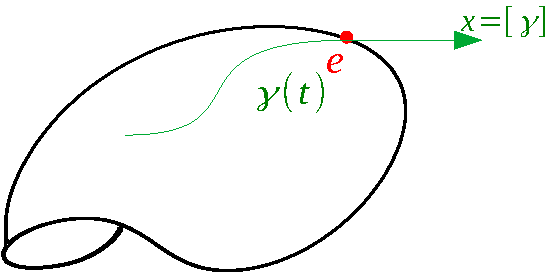
\includegraphics{images/abstract_question.pdf}
    \caption*{}
    \labfig{abstract_question}
\end{marginfigure}
\begin{align*}
    \gamma:(-\varepsilon,+\varepsilon)&\xrightarrow[]{}G\\
    t&\mapsto\gamma(t)
\end{align*}
Then we can conjugate this guy and, since $G$ is a group, this is in $G$ for every $t$; let us call this path
\[
\mu(t)=A\gamma(t)A^{-1}\in G \quad \forall t
\]
It is smooth because it is the composition of a smooth path with constant things, then 
\[
\mu(0)=e\quad \Rightarrow \quad [\mu]\in T_eG=\mathfrak{g}
\]
So what happens is that the equivalent class of $\mu$, which we might thing as a derivative, but it is not a derivative in the sense of the limit of the incremental ratio $[\mu]=\dv{t}(A\gamma(t)A^{-1})\Bigr|_{\substack{t=0}}$ replaces $AXA^{-1}$ which appears in 2) for matrix Lie groups.
\begin{proof}
\underline{\textbf{Existence}} \raisebox{-\mydepth}{{
\includegraphics[height=1.2\baselineskip]{images/lamp.png}}} Idea: we use what we know about \textbf{one-parameter subgroups} and their \textbf{unique generators}.

Choose $X\in\mathfrak{g}$, and define:
\[
A(t):=\underset{\mathclap{\tikz \node {$\uparrow$} node [below=1ex] {\footnotesize  Lie group hom};}}{\Phi}\left(e^{tX}\right) \quad \left| \quad \begin{cases}
A(0)=\mathbb{1}\\
A(t+s)=A(t)A(s)\\
A(\;):t\mapsto\Phi(e^{tX})\quad\ \text{\parbox{4 cm}{\centering is continuous because exp and $\Phi$ are $C^\infty$-continuous}}
\end{cases}
\right.
\]
As every one-parameter subgroup, it has a \textbf{unique generator} $Z$ such that
\[
A(t)=e^{tZ} \qquad \textrm{we define }\quad\phi(X):=Z
\]
In particular, it happens that
\[
\star\qquad\Big|\Big|\quad\Phi\left(e^{tX}\right)=A(t)=e^{t\phi(x)} \quad \forall\;t\in\mathbb{R}
\]
The fact that it is equal for every $t$, it will draw to many conclusions. Let us see if it satisfies all the claimed properties. First of all, by setting $t=1$, we have (D).

Second, \underline{\textbf{Linearity}}:
\renewcommand{\labelenumi}{\Roman{enumi})}
\begin{enumerate}
    \item $\phi(sX)=s\phi(X)$? This is easy, because
    \[
    e^{t\phi(sX)}=\Phi(e^{t(sX)})=e^{ts\phi(X)}
    \]
    By differentiating at $t=0$, we got the property.
    \item (\textit{Additivity}) We want to prove $\phi(X+Y)=\phi(X)+\phi(Y)$?
    
    Basically we are relating the exponential of the sum to the exponential of the sum of the images, and this is not completely obvious: we have to pass through the Lie product formula [\refthm{Lie-prod-form}].
    \WithArrowsOptions{displaystyle}
    \[
    \begin{WithArrows}
    e^{t\phi(X+Y)}\overset{(\textrm{D})}{=}\Phi(e^{t(X+Y)})&\overset{\mathclap{\tikz \node {$\downarrow$} node [above=1.25ex] {\footnotesize Lie product formula};}}{=}\Phi\left[\lim_{m\to+\infty}\left(e^{\frac{t}{m}X}e^{\frac{t}{m}Y}\right)^m\right]=\Arrow{$\Phi$ is \textbf{continuous group hom}}\\
    &=\lim_{m\to+\infty}\left[\Phi\left(e^{\frac{t}{m}X}\right)\Phi\left(e^{\frac{t}{m}Y}\right)\right]^m=\Arrow{(D)+I)}\\
    &=\lim_{m\to+\infty}\left(e^{\frac{t}{m}\phi(X)}e^{\frac{t}{m}Y}\right)^m=\Arrow{Lie product formula }\\
    &=e^{t\left(\phi(X)+\phi(Y)\right)}
    \end{WithArrows}
    \]
    So we got $e^{t\phi(X+Y)}=e^{t\left(\phi(X)+\phi(Y)\right)}\quad \forall\;t\in\mathbb{R}$. By differentiation at $t=0$, we get {\color{red}$\phi(X+Y)=\phi(X)+\phi(Y)$}.
\end{enumerate}
As promised, there exists such a map, now we have to prove that it is unique.

\underline{\textbf{Uniqueness}}: suppose $\exists\ \Tilde{\phi}:\mathfrak{g}\to\mathfrak{h}$ which is $\mathbb{R}$-linear and satisfies the defining property (D). Then we have (starting from $\Phi(e^{tX})$):
\[
e^{t\Tilde{\phi}(X)}\overset{(\textrm{D})}{=}\Phi(e^{tX})=e^{\phi(tX)}=e^{t\phi(X)}
\]
So we have that $e^{t\Tilde{\phi}(X)}=e^{t\phi(X)} \quad \forall\;t\in\mathbb{R}$. By differentiating at $t=0$, we obtain {\color{red}$\Tilde{\phi}(X)=\phi(X)$} for every $X\in\mathfrak{g}$, hence $\Tilde{\phi}\equiv \phi$.

\underline{\textbf{Additional properties}}:
\renewcommand{\labelenumi}{\arabic{enumi})}
\begin{enumerate}
\item
    \WithArrowsOptions{displaystyle}
    \[
    \begin{WithArrows}
    e^{{\color{red}t}\phi(AXA^{-1})}&\overset{(\textrm{D})}{=}\Phi(e^{A(tX)A^{-1})}=\Arrow{We proved that exp.\\ is well behaved with resp. to conj.}\\
    &=\Phi(Ae^{tX}A^{-1})=\Arrow{Homorphism}\\
    &=\Phi(A)\Phi(e^{tX})\Phi(A^{-1})=\Arrow{$\Phi$ is a group homorphism}\\
    &=\Phi(A)\Phi(e^{tX})\Phi(A)^{-1}=\Arrow{(D) + linearity in $t$}\\
    &=\Phi(A)e^{{\color{red}t}\phi(X)}\Phi(A)^{-1}
    \end{WithArrows}
    \]
    By taking the first and the last term of this chain of equalities and differentiating at zero, $\dv{t}\left(\dots\right)\big|_{t=0}$, we conclude:\marginnote{Applying the Leibniz rule, the two guys on the side are constant (the derivative is zero), so we have only the derivative of the factor in the middle, which is $\phi(X)$}
    \[
    \phi(AXA^{-1})=\dv{t}\left(\Phi(A)e^{t\phi(X)}\Phi(A)^{-1}\right)\big|_{t=0}\underset{\mathclap{\tikz \node {$\uparrow$} node [below=1ex] {\footnotesize Leibniz rule };}}{=}\Phi(A)\phi(X)\Phi(A)^{-1}
    \]
    \item $\phi(\comm{X}{Y})=\comm{\phi(X)}{\phi(Y)}$? We want again to relate something which is in the linear space (the commutator) to something in the group. The idea is that the commutator is just the infinitesimal form of the action by conjugation.\marginnote[-15mm]{This is why commutators do appear so often in QM, because we conjugate with something (e.g. time evolution) and then we look at the infinitesimal form of this action and we will get $i$ times the commutator of $H$ with the observable we are interested in. Remember that we do not have the $i$ because of this schizophrenic between mathematicians and physicist.} Therefore, the relevant formula is:
    \[
    {\color{red}XY-YX=\dv{t}\left(e^{tX}Ye^{-tX}\right)\big|_{t=0}} \qquad \Big|\Big| \quad \star
    \]
    Then we consider this guy:%\marginnote{The derivative is the limit of the incremental ratio: $\phi$ is continuous, therefore we can bring the limit outside; but $\phi$ is also linear, then the incremental ratio also goes outside, so to speak
    
    %We recall that every linear operator in finite dimensional space is continuous}
    \WithArrowsOptions{displaystyle}
    \[
    \begin{WithArrows}
    \phi(XY-YX)&=\phi\left(\dv{}{t}\left(e^{tX}Ye^{-tX}\right)\big|_{t=0}\right)=\Arrow{$\phi$ is \textbf{linear}\\hence \textbf{continuous}}\\
    &=\dv{t}\phi\left(e^{tX}Ye^{-tX}\right)\big|_{t=0}=\Arrow{Additional\\property 1)}\\
    &=\dv{}{t}{\color{red}\Phi(e^{tX}})\phi(Y){\color{red}\Phi(e^{-tX})}\big|_{t=0}=\Arrow{Homomorphisms preserve\\the inverse}\\
    &=\dv{}{t}{\Phi(e^{tX}})\phi(Y){\Phi(e^{+tX})^{-1}}\big|_{t=0}=\Arrow{(D)}\\
    &=\dv{}{t}\left(e^{t\phi(X)}\phi(Y)e^{-t\phi(X)}\right)\big|_{t=0}=\Arrow{This is the infinitesimal form\\of a conjugation}\\
    &=\phi(X)\phi(Y)-\phi(Y)\phi(X)
    \end{WithArrows}
    \]
    \item From the property:
    \[
    \Phi(e^{tX})=e^{t\phi(X)} \qquad \forall\;t\in\mathbb{R}
    \]
    We recognize that:\marginnote{We are using mixed notation}
    \[
    {\color{red}\phi(X)=\dv{}{t}\Phi(e^{tX})\big|_{t=0}=\dd\Phi\big|_{e}(X)}
    \]
    But the map $t\mapsto e^{tX}=\gamma(t)$ is a path in $G$ which is smooth and
    $\begin{cases}
    \gamma(0)=\mathbb{1}\\
    \Dot{\gamma}(0)=X
    \end{cases}$
\end{enumerate}
\end{proof}
Let us see an example (details are left as an exercise, they are in \sidecite{Hall2015_Ch3})
\begin{example}\marginnote{It is not a starred exercise because the solution it is already in the book.}
2-covering $\textrm{SU}(2)\to\textrm{SO}(3)$. Recall that we constructed a \textbf{Lie group homomorphism}, which was surjective but not injective:
\[
\begin{split}
\Phi:\textrm{SU}(2)&\twoheadrightarrow\textrm{SO}(V)\cong\textrm{SO}(3)\\
U&\mapsto\Phi_{U}
\end{split}
\]
with $V=\Bqty{X\in\textrm{Mat}(2,\mathbb{C}):X^\ast=X,\tr(X)=0}=i\textrm{SU}(2)$. And the $\Phi_U(X)$ was defined by conjugation:
\[
\Phi_U(X)=UXU^{-1}
\]
This is a Lie group homomorphism; our theorem tells us that it induces a Lie algebra homomorphism. \underline{Exercise:} compute the \textbf{induced} Lie algebra homomorphism. This will be a map:
\[
\phi:\mathfrak{su}(2)\to\mathfrak{so}(3)
\]
and check that $\phi$ is actually an \textbf{\underline{iso}-morphism}, i.e.it is bijective.

\underline{Ref:} Hall \cite{Hall2015_Ch3}

Let us sketch what is the idea:
\begin{enumerate}
    \item Choose a linear basis in $\mathfrak{so}(3)$ and $\mathfrak{su}(2)$. A convenient choice is, in $\mathfrak{so}(3)$,  the generator $F_1$ around the first axis:\marginnote{The generator will be the derivative at time $t=0$ of $R_(\theta)$}
    \[
    R_1(\theta)=\left(\begin{array}{c:cc}
    1 & 0 & 0 \\
    \hdashline
    0 & \cos\phi & -\sin\phi \\
    0 & \sin\phi & \cos\phi
    \end{array}\right) \quad \Rightarrow \ F_1=
    \left(\begin{array}{c:cc}
    0 & 0 & 0 \\
    \hdashline
    0 & 0 & -1 \\
    0 & 1 & 0
    \end{array}\right)
    \]
    and do the same for $F_2$ and $F_3$. Then check that every $F_j$ is in the Lie algebra $F_j\in\mathfrak{so}(3)$ (it is obvious by contraction) and that they are linearly independent;
    \item find the pre-images $F_j=\phi(E_j)$;
    \item check that $\phi$ maps basis into basis.
\end{enumerate}
\end{example}
Even tough all of this is in the book of Brian Hall, the professor suggests a variation of the theme since he does not like the way Brian Hall parameterize the space $V$. Indeed, in the department of Physics it would be much more natural to use the Pauli's matrices.
\begin{starredExercise}[Variation on the theme by Pauli] Notice that our space $V$ is just the Lie algebra of physicists, with our notation: $V=i\mathfrak{su}(2)$. Hence, a canonical basis %\marginnote[-2mm]{The plural of \textit{base} is \textit{\href{https://en.wiktionary.org/wiki/base}{bases}}}
in $V$ is constructed via \textbf{Pauli matrices}\index{Pauli matrices}:\marginnote[2mm]{When a matrix is like $\sigma_1$ and $\sigma_2$ it is said to be \textit{\href{https://en.wikipedia.org/wiki/Main_diagonal}{off diagonal}} (English) \textit{\href{https://it.wikipedia.org/wiki/Diagonale_principale}{anti-diagonale}} (Italian)}
\[
\sigma_1=\mqty(\admat[0]{1,1}) \quad \sigma_2=\mqty(\admat[0]{-i,i}) \quad \sigma_3=\mqty(\dmat[0]{1,-1})
\]
Check that $\Tilde{E}_j=\frac{i}{2}\sigma_j$ for $j\in\Bqty{1,2,3}$ is a basis for $\mathfrak{su}(2)$. Now we can parameterize $X\in V$ in a natural way, as
\[
X=\sum_{j=1}^3 x_j\sigma_i=\mqty(x_3 & x_1-ix_2 \\ x_1+ix_2 & -x_3)
\]
Then everything goes the same way as before (by conjugation we get a Lie group homomorphism).
\end{starredExercise}
% INIZIO LEZIONE 19 12/05/2022
% 1:01:00
\end{document}